\documentclass{article}

%\usepackage[utf8]{inputenc}
%\usepackage[T1]{fontenc}
\usepackage[frenchb]{babel}
\usepackage{lmodern}
\usepackage{fullpage}
\usepackage[normalem]{ulem}
\usepackage{epigraph}
\usepackage{listings}
\usepackage{graphicx}
\usepackage{textcomp}
\usepackage{dialogue}

\title{Réseau et administration système}
\author{boré uk}
\date{\today}

\begin{document}
\maketitle{}

\section{Administration réseau : iptables}
Sous GNU/Linux, une seule commande ici nous interesse: \emph{iptables}.\\
Cette commande permet d'effectuer \textbf{3 types de traitements}:
\begin{itemize}
\item{\textbf{Filtrer}, c'est a dire déterminer quels paquets seront acceptés ou pas \emph{(filter)}}
\item{\textbf{Translater des adresses}: une seule adresse ip publique pour plein d'adresses ip privées \emph{(nat)}}
\item{\textbf{Modifier les entetes de paquets}, mais ici on s'en fout \emph{(mangle)}}
\end{itemize}

La partie la plus importante du côté réseau concerne le \textbf{filtre}. Ainsi, on va commencer par ça.

\subsection{Filtrer les paquets}
\begin{center}
\begin{verbatim}
iptable -t filter [option iptable] [chaine] [option de filtrage] --jump [action]
\end{verbatim}
\end{center}

Pour filtrer les paquets, on va agir sur la table \emph{filter}. Ainsi, toutes les commandes \emph{iptable} commenceront de la manière suivante:
\begin{verbatim}
iptable -t filter
\end{verbatim}
Jusque là, rien de compliqué. De plus, dans la plupart des cas, on va chercher à \textbf{-A}jouter des règles par rapport à celles existantes. Du coup, on peut même dire que la plupart des commandes \emph{iptable} commenceront de cette façon:
\begin{verbatim}
iptable -t filter -A
\end{verbatim}
Pour votre gouverne, sachez qu'\emph{iptables} accepte d'autres options: on peut \textbf{supprimer} une règle (\emph{-D}), \textbf{tout supprimer} (\emph{-F}), ...

\paragraph{}
Maintenant, il faut voir qu'est-ce qu'une chaine et quels sont les chaines disponibles.\\
Une chaine définit en fait quels seront les paquets affectés par notre filtrage. Il existe 3 chaines:
\begin{itemize}
\item{\textbf{INPUT}, c'est à dire les paquets \textbf{entrants} à \textbf{destination de l'hôte}.}
\item{\textbf{OUTPUT}, c'est à dire les paquets \textbf{sortants} provenant \textbf{directement de l'hôte}.}
\item{\textbf{FORWARD}, c'est à dire les paquets \textbf{transitants} par l'hôte.}
\end{itemize}


\paragraph{}
On a notre chaine, à présent on aimerait bien agir dessus. On a 4 actions possibles sur ces chaines:
\begin{itemize}
\item{\textbf{ACCEPT}, les paquets continuent leur petit bonhomme de chemin.}
\item{\textbf{DROP}, les paquets sont ignorés}
\item{\textbf{REJECT}, les paquets sont ignorés et l'expéditeur est prévenu}
\item{\textbf{LOG}, on enregistre toutes les entrées/sorties de paquet dans un fichier log}
\end{itemize}


\paragraph{}
On peut maintenant agir sur nos chaines. \textsc{super.} \\
Vous comprendrez qu'agir sur \emph{tous les paquets}, ce n'est pas vraiment précis, mais heureusement, il existe des options de filtrage.\\
Un petit rappel du fameux modele \textsc{OSI}: \\
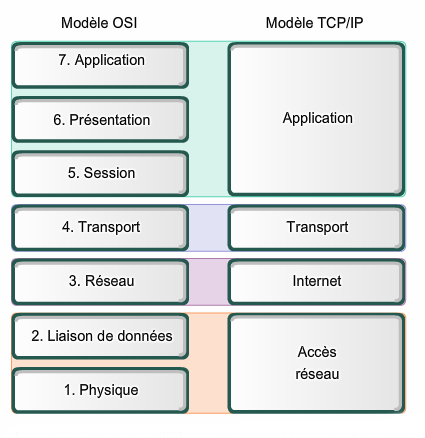
\includegraphics[scale=0.5]{osi.png}

Il existe 3 types d'options de filtrage, du plus généraliste au plus précis, qui peuvent s'utiliser ensemble:
\begin{itemize}
\item{Les filtrages sur \textbf{Trames}, qui correspond au niveau 2 du modele OSI. On agit sur les interfaces réseaux;}
\item{Les filtrages sur les \textbf{paquets ip}, c'est à dire la couche 3 du modele OSI. On agit ici par rapport aux adresses ip sources et destinations mais aussi aux protocoles (tcp/udp/icmp) utilisés par les paquets;}
\item{Les filtrages sur les \textbf{paquets tcp/udp}, c'est à dire la couche 4 du modele OSI. On agit par rapport aux ports sources et destinations, et à l'état de la connexion.}
\end{itemize}

\paragraph{Filtrage sur trames}.\\
Il existe deux options: \emph{--in-interface} [nom d'interface] et \emph{--out-interface} [nom d'interface].\\
\emph{--in-interface} désigne l'interface par laquelle les paquets \textbf{entrent} (l'hôte reçoit alors des paquets) et, de la même manière, \emph{--out-interface} désigne l'interface par laquelle les paquets \textbf{sortent} (l'hôte envoie alors des paquets).

\paragraph{Filtrage sur paquets ip}
Ici, on sera un peu plus précis.\\
On peut préciser l'adresse ip de l'expediteur (\emph{--source} [adresse ip]), ou du destinataire (\emph{--destination} [adresse ip]) ainsi que le protocole affecté par le filtrage (\emph{--protocol} [tcp/udp/tcmp/all]).

\paragraph{Filtrage sur paquets tcp/udp}.\\
On précise ici les ports expediteur (\emph{--source-port} [port]) ou port destinataire (\emph{--destination-port} [port]) affectés au filtrage. On peut aussi préciser les types de connexion concernés par le filtrage avec \emph{-m state --state} [NEW/ESTABLISHED/RELATED].

\subsection{Exemples commentés}
\begin{verbatim}
# supprime toutes les regles mais garde les existantes
iptables -t filter -F
# tous les paquets entrants par l'interface eth0 à destination de l'hote sont acceptés
iptables -t filter -A INPUT --in-interface eth0 --jump ACCEPT
# tous les paquets à destination de 192.168.30.45 de la part de l'hote sont jetés
iptables -t filter -A OUTPUT --destination 192.168.30.45 --jump DROP
# tous les paquets provenant de l'hote depuis le port 80 est accepté
iptables -t filter -A OUTPUT --protocol tcp --source-port 80 -jump ACCEPT
\end{verbatim}

\subsection{Translation d'adresses: NAT}
La translation d'adresses permet en fait d'utiliser \textbf{1 adresse ip publique} pour représenter \textbf{plusieurs machines}.  En fait, le serveur va "faire correspondre" un port sur son adresse ip à une adresse du réseau privé.\\
Sous GNU/Linux, on peut effectuer 3 actions différentes:
\begin{itemize}
\item{Masquer l'adresse ip de l'emetteur par l'adresse ip d'une interface du serveur (\emph{Masquerade}) - POSTROUTING}
\item{Changer l'adresse ip de l'emetteur par une adresse fixe spécifiée (\emph{SNAT}) - POSTROUTING}
\item{Changer l'adresse ip du destinataire par une adresse fixe spécifiée (\emph{DNAT}) - PREROUTING}
\end{itemize}
Il faut savoir qu'enfin, il existe 2 étapes bien distinctes, \emph{POSTROUTING} et \emph{PREROUTING}. Le \emph{POSTROUTING} concerne les paquets qui arrivent depuis l'exterieur vers le serveur, et qui sont destinés à une machine du réseau interne, alors que le \emph{PREROUTING} concerne les paquets envoyés depuis le réseau interne vers l'exterieur.\\
C'est pas très clair? Regardons l'exemple commenté:
\begin{verbatim}
# tous les paquets sortant par l'interface ppp0 pour le reseau interne 
# auront l'adresse ip du serveur
iptables -t nat -A POSTROUTING --out-interface ppp0 --jump MASQUERADE
# les paquets concernés sont les mêmes qu'au dessus
# sauf que cette fois ils auront l'adresse ip xxx.xxx.xxx.xxx
iptables -t nat -A POSTROUTING --out-interface ppp0 --jump SNAT --to-source xxx.xxx.xxx.xxx
\end{verbatim}

\section{Administration système: gestion des utilisateurs}
Il n'y a pas grand chose à ajouter par rapport au guide de Mr.\textsc{Lacour}.\\
Hmm, non franchement, je vois pas.\\
Rien à ajouter en fait.\\

\begin{center}
je me suis fait \textsc{preshot}
\end{center}

\end{document}